\chapter{Methodology and development} \label{chapter3}

This chapter is the crux of the entire dissertation report and goes into all the nitty-gritty details of how the entire project with all its internal components is being developed.

\vspace{-0.1in}
\section{Video data} \label{vid_data}

The entirety of the video data was procured from a company called \href{clipbyte.com}{Clipbyte} which happens to be a premier Indian broadcasting and analysis corporation responsible for broadcast/telecast management as well as dedicated analysis of various broadcasts. It also tends to various other organisations which may need this data. \par

SEBI gave the contract to Clipbyte for providing videos of NEWS shows across a span of one and a half years and a total of $7$ NEWS shows. A summary of the entire data made available to SEBI at an undisclosed contract amount is enlisted below.

\begin{table}[h]
 \def\arraystretch{1.5}
 \centering
 \caption{Summary of videos available}
 \begin{tabular}{|c|c|}
  \hline
  NEWS show & Approximate no.\\
  \hline
  Buy Now Sell Now & $435$                   \\
  \hline
  Pehla Sauda & $435$                   \\
  \hline
  NSE Closing Bell & $435$                   \\
  \hline
  Bazaar Morning Call & $435$                   \\
  \hline
  Midcap Bazaar & $435$                 \\
  \hline
  Stock 20-20 & $326$                \\
  \hline
  Weekly Roundup & $37$              \\
  \hline
 \end{tabular}
 \label{tab:news_shows_acquired}
\end{table}

The amount of video data (primarily intended for bulk processing) amounts to roughly $1.08$ Tb in size and roughly $2137$ videos ranging from as small as $250$ Mb to videos of special broadcasts amounting to excess of $900$ Mb. The data was first loaded onto an intermediate server and then finally onto the state of the art SEBI Datalake server which is essentially a cloud platform. Later, the videos are fetched as required from the Datalake server itself for further processing. The current analysis is being done from scratch on the NEWS show Midcap Bazaar from the channel ZEE NEWS using sophisticated YoLov4 models and appropriate OCR engines. The data available only from this show is shown at a glance in the following table. The data available from other NEWS shows have a similar scale although they have not been shown here for convenience.

\begin{table}[h]
 \def\arraystretch{1.5}
 \centering
 \caption{Summary of video frames from Midcap Bazaar}
 \begin{tabular}{|c|c|}
  \hline
  Parameter & Number\\
  \hline
  Total videos & $266$                   \\
  \hline
  Total frames & $8584623$                   \\
  \hline
  Average frames per video & $32273$                   \\
  \hline
  Total frames in consideration @ FPS rate & $343371$                   \\
  \hline
  Average frames in consideration per video & $1291$                   \\
  \hline
  Total size of dataset & $5000$                   \\
  \hline
 \end{tabular}
 \label{tab:vid_data_tab}
\end{table}

\section{Data annotation and preparation}

As would be obvious from the above table, the reason for mentioning FPS rates and the average total number of frames available after filtering at the FPS rate is because only these frames would be available for the creation of a dataset as mentioned in the next section. Hence filtering is done @ $25$ FPS to obtain only $25$\textsuperscript{th} of the frames available originally. How much of these would be leading to the actual training and testing data is described in the following sections. \par

\subsection{Annotation}
This single-handedly is the biggest challenge in the entire project. Irrespective of the version of the YoLo framework being used, a large part of the efforts are concentrated on the creation of massive annotated datasets. The typical annotation involves marking out appropriate bounding boxes on regions of interest i.e. ROIs (as would be described in the subsequent sections) and labelling them appropriately in video frames. A typical broadcast which could be as small as $10$ mins. will lead to as many as $3000$ video frames which only after filtering as mentioned in the previous section need to be marked appropriately. This is a laborious task that has been simplified to some extent by the availability of readymade software like \href{https://roboflow.com/annotate}{Roboflow} \cite{rb2022}. \par

However, as told previously in the section \ref{mod_guides}, our dataset should be varied enough to develop or train a model which is robust to a variety of situations that could be encountered while parsing (a) frame(s) of a video from any NEWS show. Typical edge cases which must be looked at are enumerated below.
\begin{enumerate}
 \item In NEWS show broadcasts, it is common to have minor transitions between subsequent frames, this leads to intermediate blurring and de-blurring of important regions of interest. Our model should be in a position to identify them.
 \item The recommendations being given are available in a variety of formats with a variety of spatial arrangements. All should be annotated but should be labelled with the \textbf{same class}.
 \item Sometimes ROIs appear in the same way excepting their overall scale, they should be detected exactly in the same way as if it was their original size or scale.
\end{enumerate}
Following is an illustration of the annotation section of the Roboflow software.

\begin{figure}[h]
  \centering
  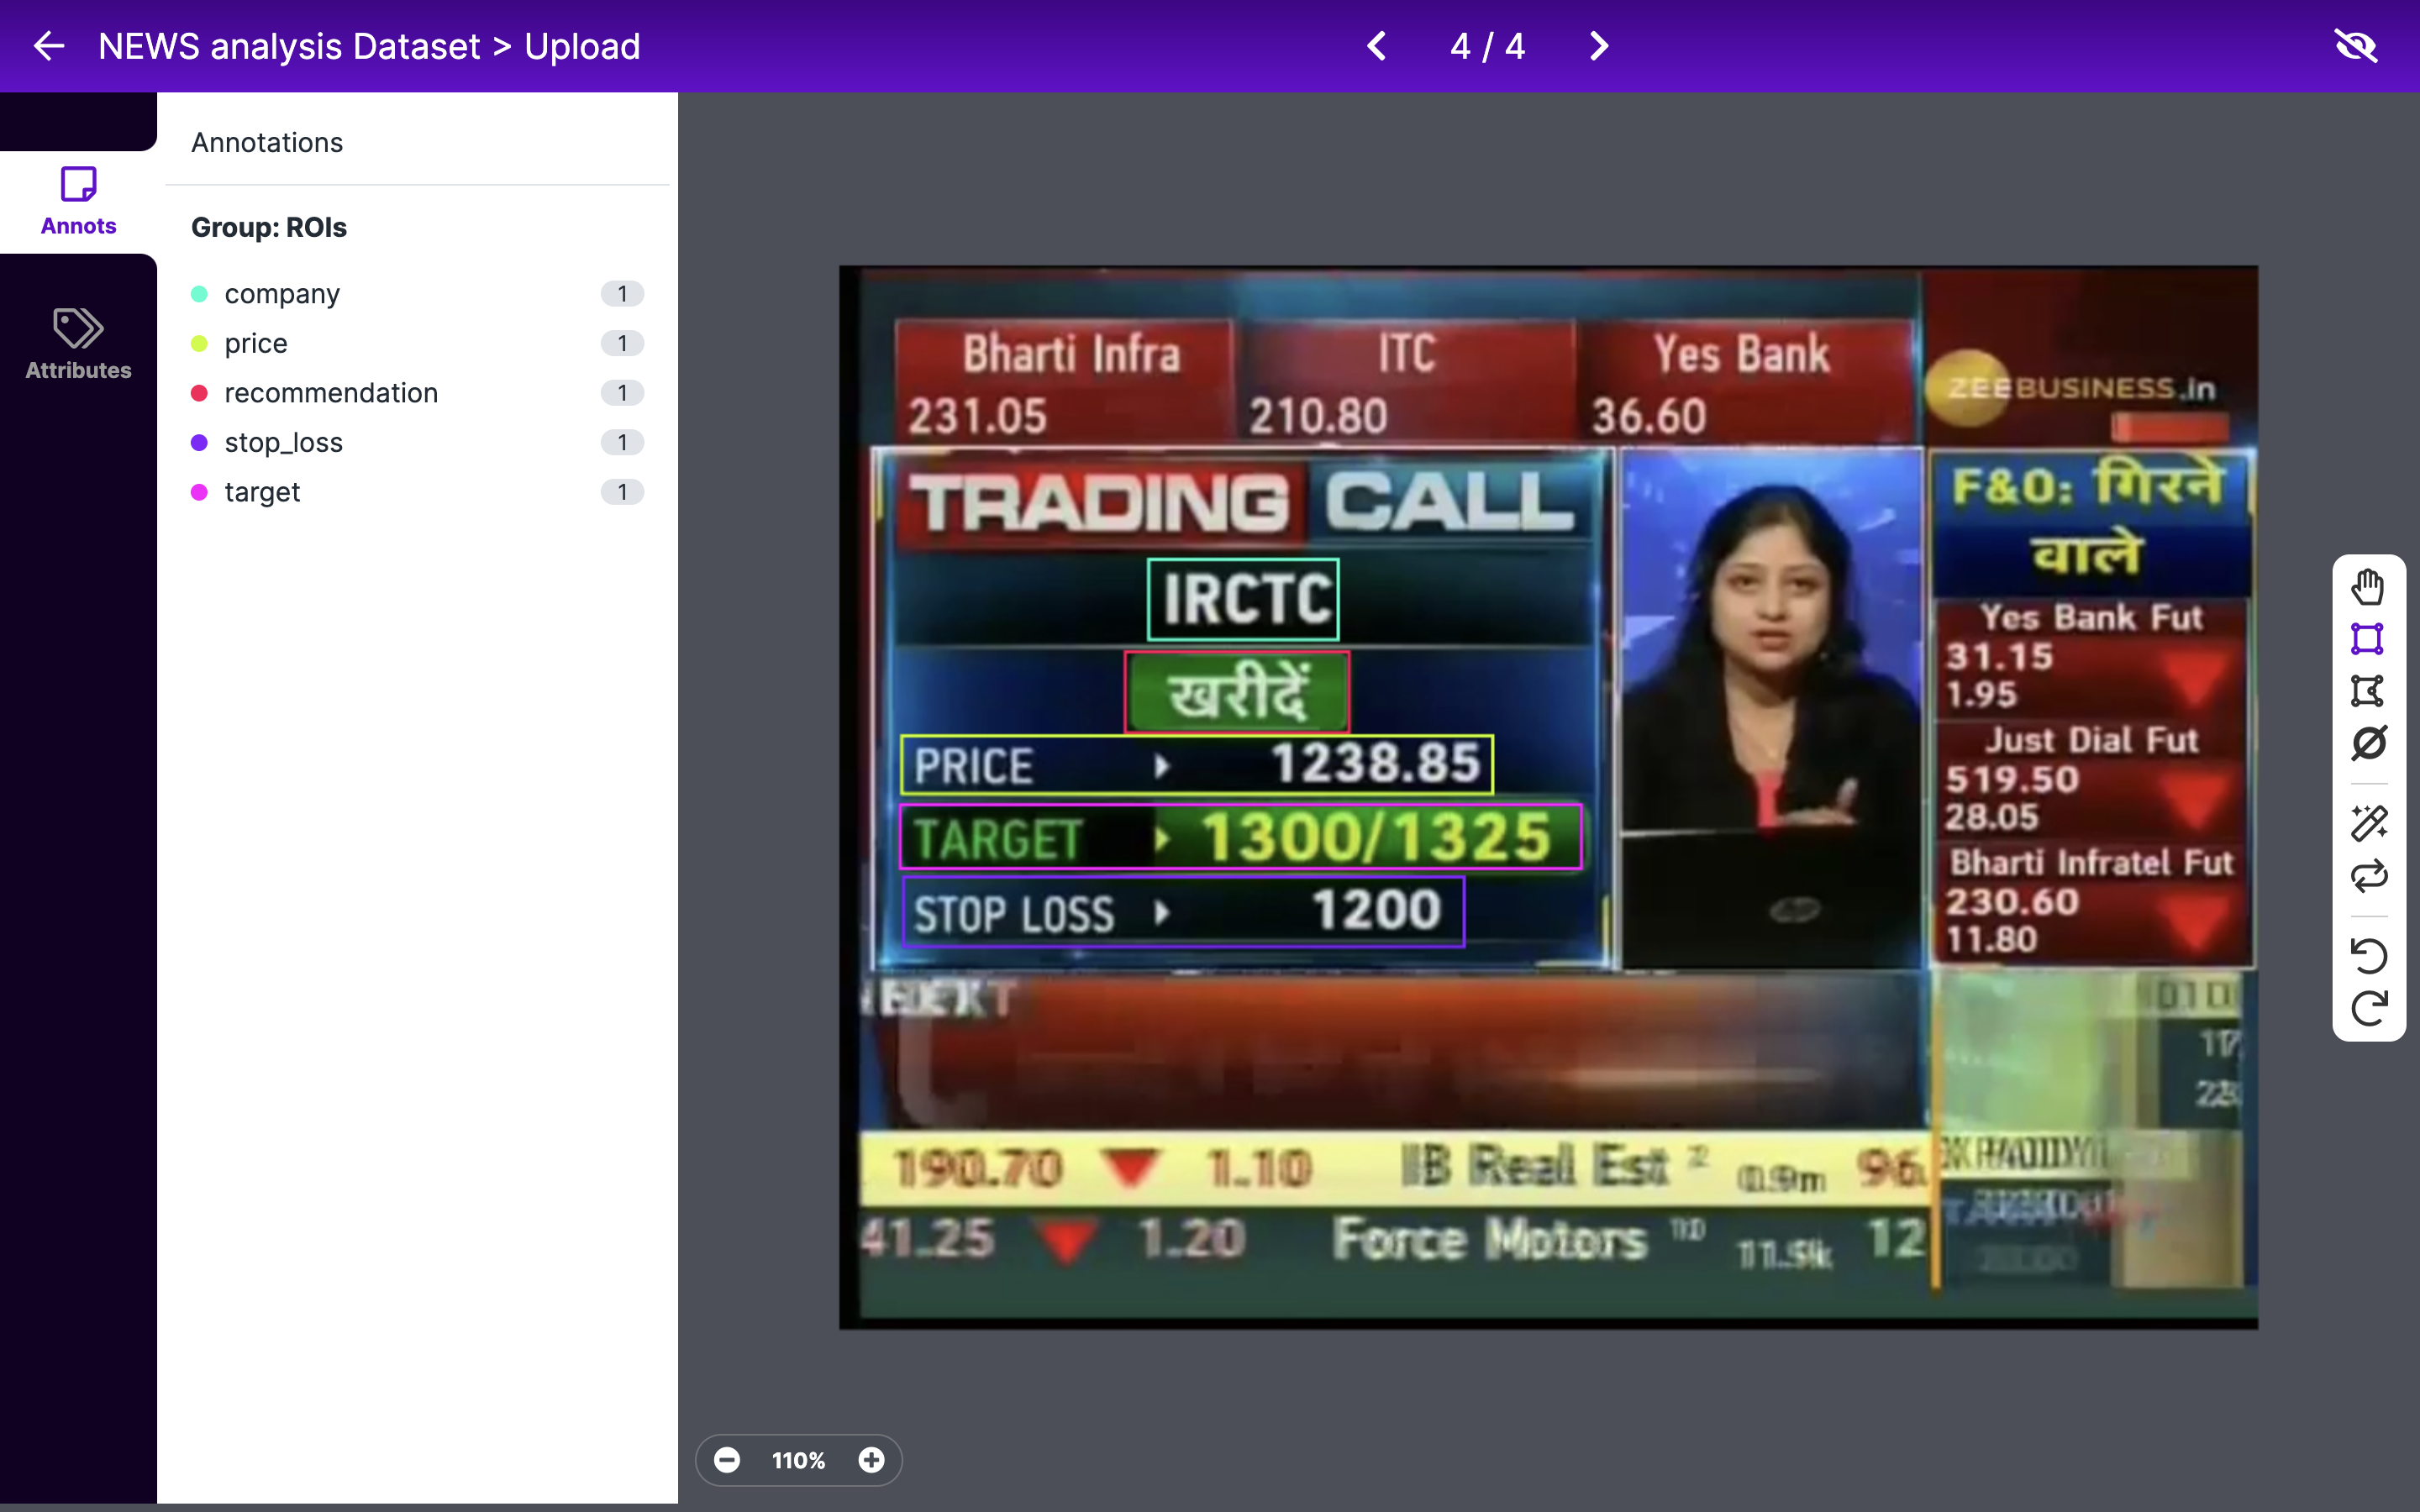
\includegraphics[scale=0.35]{chapter3/annotated_frame.png}
  \caption{The annotation screen in Roboflow clearly showing the bounding boxes made on a video frame and the appropriate classes listed on the left}
  \label{fig:annot_frame}
\end{figure}

\subsection{Data preparation for training and testing} \label{train_test}
Now we are going to boil down to the exact numbers involved in the training and testing dataset which would be summarised below. But before that, it should be noted from the table \ref{tab:vid_data_tab}, that the total images in the dataset are selected as $5000$. We can now write down a generic formula for the proportion of frames being taken from a video for annotation. Let $f_i$ be the number of frames obtained from the $i$\textsuperscript{th} video after filtering at the FPS rate and let $N$ be the total number of frames obtained across all videos in the dataset after filtering @ FPS rate i.e. $N = \sum f_{i}$. Then the proportion of its frames in the final dataset would be $\boldsymbol{F_{i} = \frac{f_{i}}{N}}$. \par

Apart from that, to adhere to the guidelines given in section \ref{mod_guides} and the edge cases described in the previous section, we need to generate a version of the dataset with each image going through a couple of additional processing steps. Such types of operations substantially increase model performance as well as drastically decrease inferencing times \cite{Joseph2021} \cite{Dwyer2020}. The operations are further divided into two parts namely \textbf{pre-processing} and \textbf{augmentation}.  The image pre-processing operations used are \textit{Resize} and \textit{Filter null}. The augmentation operations which were used are all bounding box augmentations such as \textit{crop}, \textit{blur}, \textit{brightness}, \textit{exposure} and \textit{noise}. Following is the final summary of our dataset for training and testing for a single NEWS show about its analysis as detailed in section \ref{yv4}.

\begin{table}[h]
 \def\arraystretch{1.5}
 \centering
 \caption{Summary of training dataset from Midcap Bazaar. Note: the no. of negative frames being much lesser than positive frames}
 \begin{tabular}{|c|c|}
  \hline
  Parameter & Value and unit \\
  \hline
  Frame size & $768 \times 576$                    \\
  \hline
  Training & $3500$ videos                   \\
  \hline
  Validation & $1000$ videos                 \\
  \hline
  Testing & $500$ videos                   \\
  \hline
  Positive frames (upto $7$ months) & $2566$                   \\
  \hline
  Negative frames (upto $7$ months) & $382$                   \\
  \hline
 \end{tabular}
 \label{tab:vid_train}
\end{table}

This software along with giving the capabilities to annotate a variety of subjects (pictures, videos, text etc.) produces the required weights file for the Yolo framework of any version (one through five). This when combined with the appropriate {\fontfamily{qcr}\selectfont \textbf{config}} file (a file containing the complete neural network-based configuration for the YoLo framework) is almost ready for compilation i.e. training and testing. One more additional file i.e. either a {\fontfamily{qcr}\selectfont \textbf{.data}} and/or {\fontfamily{qcr}\selectfont \textbf{names.list}} file would be required which would specify the names of the classes into which classification is supposed to occur. \par

In our case, the typical class names are used in a way that they represent what content they have in a particular frame e.g. \textbf{price}, \textbf{telecast date}, \textbf{stop loss}, textbf{recommendation} etc. The performance of the overall Python script in terms of the models used and still being worked upon are discussed in the subsequent chapters.

\section{ML/DL models}

This is the \textbf{\textit{heart and soul}} of the entire project. The methodologies mentioned here are only responsible for solving the two fundamental ML problems mentioned in chapter \ref{chapter1}. The NEWS shows are bifurcated into two parts consisting of $4$ and $3$ NEWS shows respectively. The first $4$ NEWS shows are viable for analysis in section \ref{yv3} and the latter set of shows are viable for analysis as detailed in section \ref{yv4}

\subsection{YoLov3 and random forest classifiers} \label{yv3}

It should be noted that the mere usage of the YoLov3 framework didn’t give a substantial number of accurate results so the training dataset was enhanced using \textbf{random forest classifiers} to obtain a substantial increase in percentage accuracy. The logic behind this is better illustrated through the following two flowcharts.

\begin{figure}[h]
 \centering
 \begin{tikzpicture}[node distance=2cm]
  \node (input) [io] {Image data};
  \node (yolov3) [process, right of=input, xshift=2cm] {YoLov3 models};
  \node (output) [io, right of=yolov3, xshift=3cm] {Moderate accuracy};
  \draw [arrow] (input) -- (yolov3);
  \draw [arrow] (yolov3) -- (output);
 \end{tikzpicture} \\
 \vspace{1.5cm}
 \begin{tikzpicture}[node distance=2cm]
  \node (input) [io] {Image data};
  \node (yolov3) [process, right of=input, xshift=2cm] {YoLov3 models};
  \node (rf) [process, right of=yolov3, xshift=2cm] {RF classifier};
  \node (output) [io, right of=rf, xshift=3cm] {High accuracy};
  \draw [arrow] (input) -- (yolov3);
  \draw [arrow] (yolov3) -- (rf);
  \draw [arrow] (rf) -- (output);
 \end{tikzpicture}
 \caption{A flowchart representation of the two different approaches: with and wihtout random forest classifiers}
 \label{fig:not_rf_and_rf}
\end{figure}

This section has been bifurcated into two parts, the first dealing with the dataset on which the classifier was trained and the second dealing with how the actual Python script works.

\subsubsection{Random forest classifiers}
Two random forest classifiers are being used for this project i.e. one for identifying the appropriate BUY/SELL/HOLD \textbf{recommendation} and another for identifying the correct \textbf{analyst name} who is hosting the NEWS show and giving the recommendations. Important regions of interest within a particular video frame are identified and kept aside. \par

Now a reference list is used which has the analyst names inside it and corresponding to which there are several columns corresponding to a total of 784 pixels each with the labelling of either 1 or 0 telling whether the concerned pixel had a subset (or a part) of the analyst name inside it. As expected only two-three distinct analyst names are listed in the first column while the number of data entries corresponds to a total of 3425 rows. Similarly, the other classifier is trained wherein the first column deals with the recommendation while the remaining rows denote the pixels. Here there are a total of 4559 rows. The first classifier had 3000 rows for training and the latter had 4300 rows for the same. The remaining rows in each case were used for testing purposes. \par

The overall classifier model would simply take in a list of $784$ pixels obtained from an image that has been passed through a threshold value of $100$.

\subsubsection{Python script methodology}
The actual python script being long can only be described in brief. Important ROIs are targeted for different NEWS shows. Frames obtained are trimmed off at these specific coordinates. Then all these ROIs are passed into a total of $12$ different image pre-processing operations simultaneously. All of them are then passed into the concerned OCR frameworks to obtain the corresponding text inside them. The text which doesn’t go into the ML models is compared against existing NSE listings to figure out the correct company name using string matching algorithms (matching set at particular thresholds). Then the final output obtained is summarized into a proper CSV format and displayed to the end-user.

\begin{figure}[h]
  \centering
  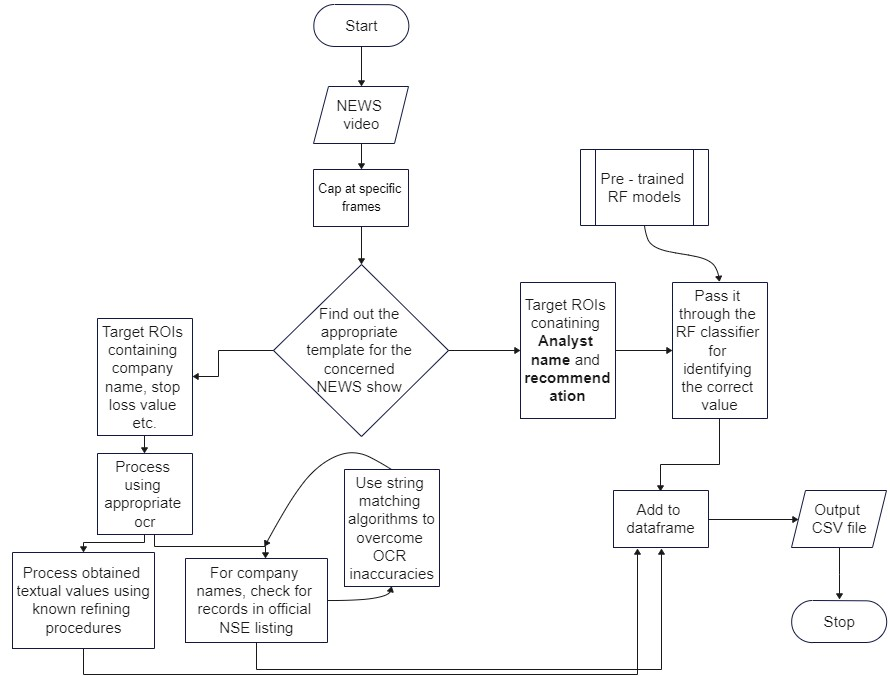
\includegraphics[scale=0.7]{chapter3/overall flow.jpeg}
  \caption{A flowchart representation of the entire methodology of the Python script}
  \label{fig:process_flow_python}
\end{figure}

\subsection{YoLov4} \label{yv4}

After the complete training of the dataset as described in the section \ref{train_test} is concluded, the execution of the {\fontfamily{qcr}\selectfont darknet.exe} command or the calling of a high-level library on a particular frame produces bounding boxes with appropriate coordinates, the class detected and the confidence score associated with each detection. There could be multiple detections in a frame, all of which would be returned. We may choose to somehow aggregate the confidence scores at the end to show an overall value of the percentage accuracy but it is completely optional. The important part of this process is \textbf{bounding box coordinates} which are obtained at the end. These would be sent into the OCR engine described in the next section.

\subsection{OCR models}

The deep learning models which follow the above YoLov4 models are the cascaded models working under the hood of the OCR engine. EasyOCR is the OCR chosen for this project, the reasons for which are described in section \ref{comp_ocr}. The two models are essentially a \textbf{text detection} model and a \textbf{language} model. It should be noted that there is only a single text detection model, however, there could be as many language detection models as you wish to detect. The common directory under which both these models would be stored is mentioned in the program as a path variable.

\begin{figure}[h]
  \centering
  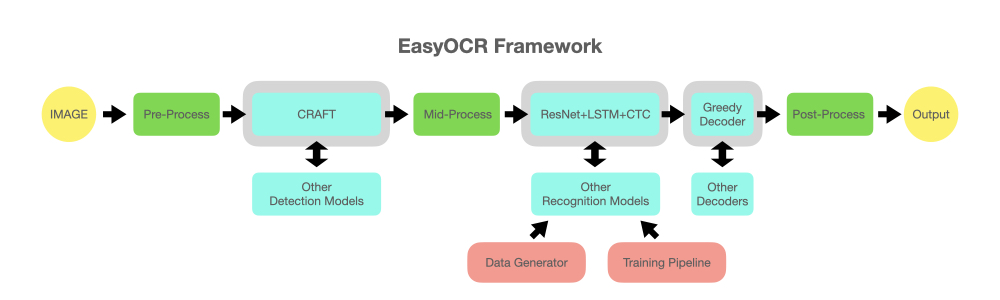
\includegraphics[scale=0.45]{chapter3/easyocr_framework.jpeg}
  \caption{The internal flow of EasyOCR}
  \label{fig:internal_ocr}
\end{figure}}

The methodology which is followed here is that the bounding box coordinates obtained from the previous step are converted to the form {\fontfamily{qcr}\selectfont [row\_start:row\_stop, column\_start:column\_stop]} which is applicable for any Python NumPy object or equivalently any image. EasyOCR then applies its capabilities only in the specific region as described by the set of converted coordinates. \par

The text detected would be having a variety of numerical values of stop-loss, target price, etc. All of them would essentially be linked to a single company (its listing symbol to be specific). This listing symbol forms the basis of creating keys in a Python dictionary which would all be unique. Any update to this dictionary would either add a key or update the values corresponding to a single key (or a listing symbol). It should be noted that the latter case is rare since analysts rarely give \textit{different} recommendations regarding the same company multiple times in a single broadcast. Then the concerned dictionary is converted to a Pandas data frame which is then finally converted to a CSV or an excel file as desired after appending a column containing a single date at the end. \par

This concludes the typical program flow for such a script. The following section describes, in brief, a difficult edge case wherein multiple recommendations may be detected in a single frame.

\subsubsection{Multiple recommendations in a frame}

Although we have not gone into the details of how the dataset on which the training is carried out in section \ref{train_test} looks like. It is known that there exist rare situations wherein multiple recommendations corresponding to distinct company shares are given in the same frame. In such cases, it is difficult to associate recommendations and other numerical values accurately with a company or its listing symbol. I have proposed a method below which is simple to follow and leads to substantial accuracy in such cases. \par

We are well aware that the multiple bounding boxes that are being returned by the YoLov4 model all lie along the same vertical axis. The only discerning feature is the limits of the bounding boxes along the $X$ - axis. Let $X_i$ and $X_j$ be the $X$ - axis limits for a detection containing a company name or its symbol. Let $x_i$ and $x_j$ be the $X$ - axis limits for a detection containing any of the following values: recommendation, target price, stop loss etc. The latter can be associated with the former if and only if either or both of the $X$ - axis limits of the latter are contained within the former. Precisely, the latter can be associated with the former if $x_{i} \geqslant X_{i}$ and (or)  $x_{j} \leqslant X_{j}$. It is driven by the reason that the latter is usually placed below the former in any NEWS show but with identical text size and width. \par

This concludes the discussion of the entire methodology involved in the project.
